\begin{exercises} 

\item \label{Ez:10.2.1}   The Heat Index, $I$, (measured in \emph{apparent degrees F}) is a function of the actual temperature $T$ outside (in degrees F) and the relative humidity $H$ (measured as a percentage).  A portion of the table which gives values for this function, $I(T,H)$, is reproduced below:
\begin{center}
\begin{tabular}{|l||r|r|r|r|} \hline
\emph{T} $\downarrow \backslash$ \emph{H} $\rightarrow$ 
	& 70 &	75 & 80 &	85  \\ \hhline{|=|=|=|=|=|}
90 & 106 & 109 & 112 & 115  \\ \hline
92 & 112 & 115 & 119 & 123  \\ \hline
94 & 118 & 122 & 127 & 132  \\ \hline
96 & 125 & 130 & 135 & 141  \\ \hline
\end{tabular}
\end{center}

				
    \ba
   	\item State the limit definition of the value $I_T(94,75)$.  Then, estimate $I_T(94,75)$, and write one complete sentence that carefully explains the meaning of this value, including its units.	
	
	\item State the limit definition of the value $I_H(94,75)$.  Then, estimate $I_H(94,75)$, and write one complete sentence that carefully explains the meaning of this value, including its units.
	
	\item Suppose you are given that $I_T(92,80) = 3.75$ and $I_H(92,80) = 0.8$.  Estimate the values of $I(91,80)$ and $I(92,78)$.  Explain how the partial derivatives are relevant to your thinking.
	
	\item On a certain day, at 1 p.m. the temperature is 92 degrees and the relative humidity is 85\%.  At 3 p.m., the temperature is 96 degrees and the relative humidity 75\%.  What is the average rate of change of the heat index over this time period, and what are the units on your answer?  Write a sentence to explain your thinking.
	
%	\item (6) Recall the given information from (b) that $I_T(92,80) = 3.75$ and $I_H(92,80) = 0.8$.  Suppose that on a day when the temperature is 92$^\circ$ with relative humidity of 80\%, at the time these data are recorded, the actual temperature is decreasing at a rate of 2 degrees per hour and relative humidity is rising at a rate of 3\% per hour.  At what instantaneous rate is the heat index changing at this time?  What are the relevant units on this rate of change?  Write a sentence to clearly explain your thinking in this problem and justify your answer.
    \ea

\begin{exerciseSolution}
\ba
   	\item The limit definition of the value $I_T(94,75)$ is
\[I_T(94,75) = \lim_{h \to 0} \frac{I(94+h,75)-I(94,75}{h}.\]
We can use a symmetric difference quotient to estimate $I_T(94,75)$:
\[I_T(94,75) \approx \frac{I(94+2,75)-I(94-2,75)}{4} = \frac{13}{4} = 3.25.\]
The number $I_T(94,75)$ tells us that if the temperature increases by $1^{\circ}$F from $94^{\circ}$F while the relative humidity remains constant at 75\%, the heat index increases by approximately $3.25^{\circ}$F. In other words, it feels approximately $3.25^{\circ}$F warmer if the temperature increases by $1^{\circ}$F from $94^{\circ}$F while the relative humidity remains constant at 75\%.
	
	\item The limit definition of the value $I_H(94,75)$ is
\[I_H(94,75) = \lim_{h \to 0} \frac{I(94,75+h)-I(94,75}{h}.\]
We can use a symmetric difference quotient to estimate $I_H(94,75)$:
\[I_H(94,75) \approx \frac{I(94,75+5)-I(94,75-5)}{10} = \frac{9}{10} = 0.9.\]
The number $I_H(94,75)$ tells us that if the relative humidity increases by 1\% from 75\% while the temperature remains constant at $94^{\circ}$F, the heat index increases by approximately $0.9^{\circ}$F. In other words, it feels approximately $0.9^{\circ}$F warmer if the relative humidity increases by 1\% from 75\% while the temperature remains constant at $94^{\circ}$F, the heat index increases by approximately $0.9^{\circ}$F.
	
	\item By definition,  
\[I_T(92,80) \approx \frac{I(91,80)-I(92,80)}{-1},\]
so 
	\[I(91,80) \approx I(92,80) - I_T(92,80) = 119-3.75 = 115.25.\]
Similarly, by definition,  
\[I_T(92,80) \approx \frac{I(92,78)-I(92,80)}{-2},\]
so 
	\[I(92,78) \approx I(92,80) - 2I_H(92,80) = 119-2(0.8) = 117.4.\]

	\item The average rate of change of the heat index over this time period will be the change in the heat index divided by the time. So the average rate of change of the heat index from 1 p.m. to 3 p.m. is 
\[\frac{I(96,75)-I(92,85)}{3-1} = \frac{130-123}{2} = 3.5 \ \frac{^{\circ}\text{F}}{\text{hour}}.\]
\ea

\end{exerciseSolution}

\item \label{Ez:10.2.1.5} Let $f(x,y) = \frac{1}{2}xy^2$ represent the kinetic energy in Joules of an object of mass $x$ in kilograms with velocity $y$ in meters per second. Let $(a,b)$ be the point $(4,5)$ in the domain of $f$.
    \ba
    \item Calculate $f_x(a,b)$.
    
    \item Explain as best you can in the context of kinetic energy what the partial derivative
\[f_x(a,b) = \lim_{h \to 0} \frac{f(a+h,b) - f(a,b)}{h}\]
tells us about kinetic energy.

    \item Calculate $f_y(a,b)$.

    \item Explain as best you can in the context of kinetic energy what the partial derivative
\[f_y(a,b) = \lim_{h \to 0} \frac{f(a,b+h) - f(a,b)}{h}\]
tells us about kinetic energy.



     \item Often we are given certain graphical information about a function instead of a rule. We can use that information to approximate partial derivatives. For example, suppose that we are given a contour plot of the kinetic energy function (as in Figure \ref{F:10.2.pd_contour}) instead of a formula. Use this contour plot to approximate $f_x(4,5)$ and $f_y(4,5)$ as best you can. Compare to your calculations from earlier parts of this exercise.  
\begin{figure}[ht]
  \begin{center}
%       \scalebox{0.5}{\includegraphics{figures/10_2_pd_contour}}
    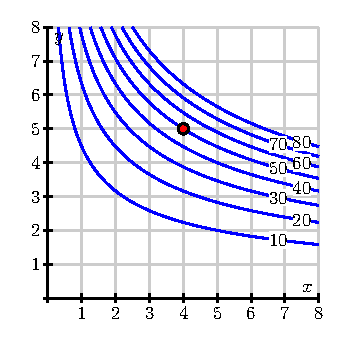
\includegraphics{figures/fig_10_2_ke_contour.eps}
    \caption{The graph of $f(x,y) = \frac{1}{2}xy^2$.}
    \label{F:10.2.pd_contour}
  \end{center}
\end{figure}
    \ea
\begin{exerciseSolution}
    \ba
    \item A straightforward calculation shows that 
\[f_x(x,y) = \frac{1}{2}y^2.\]
So 
\[f_x(a,b) = \frac{1}{2}(5^2) = 12.5.\]

    \item The value of $f_x(a,b)$ tells us that if the mass of the object increases by 1 kg from 4 kg while the velocity of the object remains constant at 5 meters per second, the kinetic energy of the object increases by approximately 12.5 Joules. 

    \item A straightforward calculation shows that 
\[f_y(x,y) = xy.\]
So 
\[f_y(a,b) = (4)(5) = 20.\]

    \item The value of $f_y(a,b)$ tells us that if the velocity of the object increases by one meter per second from a velocity of 5 meters per second while the mass remains constant at 4 kg, the kinetic energy of the object increases by approximately 20 Joules. 

		\item To approximate $f_x(4,5)$, we will use a symmetric difference quotient. That is,
\[f_x(4,5) \approx \frac{f(4+h,5)-f(4-h,5)}{2h}\]
for a suitable value of $h$. We can approximate the values of $f$ on the contour plot for $h = 1$, giving us 
\[f_x(4,5) \approx  \frac{f(5,5)-f(3,5)}{2} \approx \frac{60-40}{2} = 10.\]
Similarly,
\[f_y(4,5) \approx  \frac{f(4,6)-f(4,4)}{2} \approx \frac{65-30}{2} = 17.5.\]
These values compare reasonably well to the values of $f_x(4,5) = 12.5$ and $f_y(4,5) = 20$ obtained earlier.
    \ea

\end{exerciseSolution}

\item \label{Ez:10.2.2}    The temperature on an unevenly heated metal plate positioned in the first quadrant of the $x$-$y$ plane is given by 
$$C(x,y) = \frac{25xy+25}{(x-1)^2 + (y-1)^2 + 1}.$$
Assume that temperature is measured in degrees Celsius and that $x$ and $y$ are each measured in inches. ({\bf Note:} At no point in the following questions should you expand the denominator of $C(x,y)$.)

\ba

	\item Determine $\frac{\partial C}{\partial x}|_{(x,y)}$ and $\frac{\partial C}{\partial y}|_{(x,y)}$.  

	\item If an ant is on the metal plate, standing at the point $(2,3)$, and starts walking in a direction parallel to the $y$ axis, at what rate will the temperature he is experiencing change?  Explain, and include appropriate units.

	\item If an ant is walking along the line $y = 3$, at what instantaneous rate will the temperature he is experiencing change when he passes the point $(1,3)$?

	\item Now suppose the ant is stationed at the point $(6,3)$ and walks in a straight line towards the point $(2,0)$.  Determine the \emph{average} rate of change in temperature (per unit distance traveled) the ant encounters in moving between these two points.  Explain your reasoning carefully.  What are the units on your answer?
	

    \ea

\begin{exerciseSolution}
\ba

	\item Using the product rule from single variable calculus we have 
\[\frac{\partial C}{\partial x}|_{(x,y)} = \frac{\left((x-1)^2 + (y-1)^2 + 1\right)(25y) - (25xy+25)(2(x-1))}{\left((x-1)^2 + (y-1)^2 + 1\right)^2}\]
and
\[\frac{\partial C}{\partial y}|_{(x,y)} = \frac{\left((x-1)^2 + (y-1)^2 + 1\right)(25x) - (25xy+25)(2(y-1))}{\left((x-1)^2 + (y-1)^2 + 1\right)^2}.\]

	\item The rate at which the temperature of the place will change in the $y$ direction will be 
\[\frac{\partial C}{\partial y}|_{(2,3)} = -\frac{100}{9} \ \frac{^{\circ}\text{C}}{\text{in}}.\]
So the temperature of the plate is decreasing by $\frac{100}{9}$ $^{\circ}$C as the ant moves from the point $(2,3)$ in the direction parallel to the $y$-axis.

	\item Now $y$ is held constant, so the change in temperature at this point is 
	\[\frac{\partial C}{ \partial x}|_{(1,3)} = 15 \ \frac{^{\circ}\text{C}}{\text{in}}.\]

	\item Here we want the total change in temperature divided by the total distance traveled. This gives us the average rate of change of the temperature between the points $(6,3)$ and $(2,0)$ as
\[\frac{C(6,3)-C(2,0)}{|(6,3)-(2,0)|} = \frac{1}{\sqrt{4^2+3^2}}\left(\frac{95}{6}-\frac{25}{3}\right) = 1.5 \ \frac{^{\circ}\text{C}}{\text{in}}.\]
	

    \ea
\end{exerciseSolution}

\item \label{Ez:10.2.3}    Consider the function $f$ defined by  $f(x,y) = 8 - x^2 -  3y^2$.
				
    \ba
   	\item Determine $f_x(x,y)$ and $f_y(x,y)$.
	\item Find parametric equations in $\R^3$ for the tangent line to the trace $f(x,1)$ at $x=2$.
	\item Find parametric equations in $\R^3$ for the tangent line to the trace $f(2,y)$ at $y=1$.
	\item State respective direction vectors for the two lines determined in (b) and (c).
	\item Determine the equation of the plane that passes through the point $(2,1,f(2,1))$ whose normal vector is orthogonal to the direction vectors of the two lines found in (b) and (c).
	\item Use a graphing utility to plot both the surface $z = 8 - x^2 - 3y^2$ and the plane from (e) near the point $(2,1)$.  What is the relationship between the surface and the plane?
    \ea

\begin{exerciseSolution}
    \ba
   	\item Straightforward calculations show that 
\[f_x(x,y) = -2x \ \text{ and } \ f_y(x,y) = -6y.\]

	\item The tangent line goes through the point $(2,1)$ in the $x$-direction. The $x$ values and $z$ values change, with $f_x(2,1)$ telling us how $z$ changes while the $y$ value remains constant at 1. A set of parametric equations for this line is
\[x(t) = 2+t, \ y(t)=1, \ \text{ and } \ z(t) = f(2,1) + f_x(2,1)t = 1-4t.\]

	\item The tangent line goes through the point $(2,1)$ in the $y$-direction. The $y$ values and $z$ values change, with $f_y(2,1)$ telling us how $z$ changes while the $x$ value remains constant at 2. A set of parametric equations for this line is
\[x(t) = 2, \ y(t)=1+t, \ \text{ and } \ z(t) = f(2,1) + f_y(2,1)t = 1-6t.\]

	\item A direction vector for the tangent line in the $x$-direction is $\langle 1, 0, f_x(2,1) \rangle = \langle 1, 0, -4 \rangle$ and a direction vector for the tangent line in the $y$-direction is $\langle 0, 1, f_y(2,1) \rangle = \langle 0, 1, -6 \rangle$

	\item A normal vector $\vn$ for the plane is a vector orthogonal to the two direction vectors, so 
\[\vn = \langle 1, 0, f_x(2,1) \rangle \times \langle 0, 1, f_y(2,1) \rangle = \langle -f_x(2,1), -f_y(2,1), 1 \rangle = \langle -4, -6, 1 \rangle.\]
The plane through the point $(2,1,f(2,1)) = (2,1,1)$ with normal vector $\langle -4, -6, 1 \rangle$ has equation
\[4(x-2)+6(y-1)+(z-1) = 0 \ \text{ or } \ z = 1 - 4(x-2) - 6(y-1).\]

	\item A plot of the surface $z = 8 - x^2 - 3y^2$ and the plane from (e) near the point $(2,1)$ shows that the surface is very closely approximated by this plane for points near $(2,1)$. This is analogous to the tangent line approximation from single variable calculus. 
\ea
\end{exerciseSolution}


\end{exercises}
\afterexercises
